\section{Identification de solutions}

Au laboratoire, Enzo a trouvé un flacon sans étiquette, qui contient une solution incolore. 

\begin{center}
	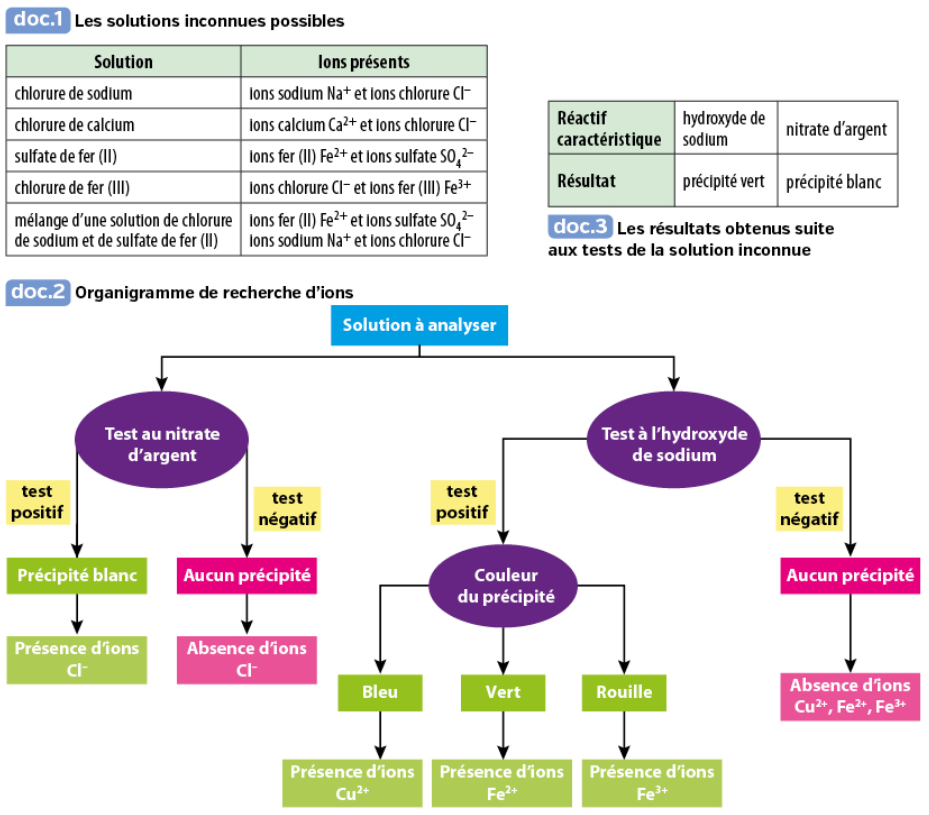
\includegraphics[scale=0.6]{img/docs}
\end{center}

\begin{questions}
	\question La solution inconnue est l'une de celles présentes dans le doc. 1. Quels tests doit-il faire pour l'identifier ? Décrire le protocole expérimental.
	
	\question Représenter un de ces tests à l'aide d'un schéma.
	
	\question D'après les résultats obtenus présentés dans le doc. 3, quels ions ont été identifiés par les tests ? 
	
	\question Quelle est la solution contenue dans le flacon ?
	
	\question Détailler la composition de chacun des ions présents dans la solution. (nombre de protons, nombre d'électrons, nombre de charges).
	
	
\end{questions}